\documentclass[12pt,a4paper,oneside]{book}
\usepackage{booktabs}
\usepackage{blindtext}
\usepackage{lipsum}
\usepackage{siunitx}

\usepackage[QX]{polski}
\usepackage[utf8]{inputenc}
\usepackage{latexsym}
\usepackage{tgpagella}
\usepackage{lmodern}
\usepackage{amsmath,amsthm,amsfonts,amssymb,alltt}
\usepackage{epsfig}
\usepackage{pdflscape}
\usepackage{caption}
\usepackage{indentfirst}
\usepackage{float}
\usepackage{graphicx}
\usepackage{biblatex}
\usepackage[nottoc]{tocbibind}
%\usepackage{showkeys}

\usepackage[x11names,dvipsnames,table]{xcolor}
\usepackage{hyperref}
\hypersetup{
pdfauthor={Roman Czapla},
colorlinks=True,
linkcolor=darkgray,  % color of internal links (change box color with linkbordercolor)
citecolor=BrickRed,  % color of links to bibliography
filecolor=Magenta,   % color of file links
urlcolor=BlueViolet}	%%pdfpagemode=FullScreen}

% diagramy, grafy itp.
\usepackage{tikz}
\usetikzlibrary{positioning}
\usetikzlibrary{arrows}
\usetikzlibrary{arrows.meta}
\usetikzlibrary{chains,fit,shapes,calc}
\tikzset{main node/.style={circle,fill=blue!20,draw,minimum size=1cm,inner sep=0pt}}


\usepackage[linesnumbered,lined,commentsnumbered, algochapter]{algorithm2e}
\SetKwFor{ForEach}{for each}{do}{end for}%
\SetKwFor{ForAll}{for all}{do}{end for}%
\newenvironment{myalgorithm}
{\rule{\textwidth}{0.5mm}\\\SetAlCapSty{}\SetAlgoNoEnd\SetAlgoNoLine\begin{algorithm}}{\end{algorithm}\rule{\textwidth}{0.5mm}}


%---------------------
\overfullrule=2mm
\pagestyle{plain}
\textwidth=15cm \textheight=685pt \topmargin=-25pt \linespread{1.3} 
\setlength{\parskip}{0pt}
\setlength\arraycolsep{2pt}
\oddsidemargin =0.9cm
\evensidemargin =-0.1cm

\captionsetup{width=.95\linewidth, justification=centering}
%---------------------


\usepackage{color}

% --------------------------------------------
% Definicja konwencji wizualnej dla kodu
%\definecolor{mygreen}{rgb}{0,0.6,0}
\definecolor{mygray}{rgb}{0.92,0.92,0.92}
\definecolor{light-gray}{gray}{0.85}
\definecolor{mymauve}{rgb}{0.58,0,0.82}
%\definecolor{myred}{rgb}{1,0,0}


\usepackage{listings}
% wspólny licznik dla figures and lislistings
\makeatletter
\AtBeginDocument{%
  \let\c@figure\c@lstlisting
  \let\thefigure\thelstlisting
  \let\ftype@lstlisting\ftype@figure % give the floats the same precedence
}
\makeatother
%----------------------------------------
\usepackage{listingsutf8}
\renewcommand{\lstlistingname}{Rys.}%{Kod \'{z}r\'{o}d\l{l}owy}
\lstset{
basicstyle=\ttfamily ,
language=python,
inputencoding=utf8/cp1250,
extendedchars=true,
numbers=left, %eller none
numberstyle=\scriptsize\color{black}\bfseries,
%frame = tb,
captionpos = rb,
backgroundcolor=\color{light-gray},
xleftmargin=\parindent,
% xrightmargin=3.5cm
showstringspaces=false,
commentstyle=\color{Red},
keywordstyle=\color{YellowOrange},
keywordstyle=[2]\color{RedViolet},
keywords={and,del,from,not,while,as,elif,global,or,with,assert,else,if,pass,yield,break,
except,import,class,exec,in,raise,continue,finally,is,return,def,for,lambda,try},
keywords=[2]{print,object,type,input,sum,min,max,int,float,str,list,dict,set,tuple},
rulesepcolor=\color{Blue},
escapeinside={<@}{@>},
stringstyle=\color{OliveGreen},
%basicstyle=\color{Black},
%morecomment=[l]\#,%
morestring=[d]{\\'},
morestring=[d]{\\"},
%morestring=[b]',%
%morestring=[b]",%
%morestring=*[d]',%
%morestring=*[d]",%
%morestring=[d]{\\'},
%morestring=**[d]{"},
%morestring=[d]{\\"},
morestring=[s]{'}{'},
morestring=[s]{"}{"},
morestring=[s]{'''}{'''},
morestring=[s]{"""}{"""},
morestring=[s]{f"""}{"""},
morestring=[s]{r"""}{"""},
morestring=[s]{f"}{"},
morestring=[s]{f'}{'},
morestring=[s]{r"}{"},
morestring=[s]{r'}{'},
morecomment=[s]{Traceback}{Error*},
literate={ą}{{\k{a}}}1
             {Ą}{{\k{A}}}1
             {ę}{{\k{e}}}1
             {Ę}{{\k{E}}}1
             {ó}{{\'o}}1
             {Ó}{{\'O}}1
             {ś}{{\'s}}1
             {Ś}{{\'S}}1
             {ł}{{\l{}}}1
             {Ł}{{\L{}}}1
             {ż}{{\.z}}1
             {Ż}{{\.Z}}1
             {ź}{{\'z}}1
             {Ź}{{\'Z}}1
             {ć}{{\'c}}1
             {Ć}{{\'C}}1
             {ń}{{\'n}}1
             {Ń}{{\'N}}1
}



% --------------------------------------------


\newtheorem{tw}{Twierdzenie}[chapter]
\newtheorem{lem}[tw]{Lemat}
\newtheorem{co}[tw]{Wniosek}
\newtheorem{prop}[tw]{Stwierdzenie}
\theoremstyle{definition}
\newtheorem{ex}{Przykład}
\newtheorem{re}[tw]{Uwaga}
\newtheorem{de}{Definicja}[chapter]



\newcommand{\bC}{{\mathbb C}}
\newcommand{\bR}{{\mathbb R}}
\newcommand{\bZ}{{\mathbb Z}}
\newcommand{\bQ}{{\mathbb Q}}
\newcommand{\bN}{{\mathbb N}}
\newcommand{\captionT}[1]{\caption{\textsc{\footnotesize{#1}}}}
\renewcommand\figurename{Rys.}

\numberwithin{equation}{chapter}
\renewcommand{\thefootnote}{\arabic{footnote})}
%\renewcommand{\thefootnote}{\alph{footnote})}

 %\usepackage[maxcitenames=3]{biblatex}
 
\usepackage[polish]{babel}
%\usepackage{biblatex}
\addbibresource{bibliografia.bib}

\newcommand{\source}[1]{Źródło: \url{#1}}
\newcommand{\customsource}[1][]{{Źródło własne #1}}
\newcommand{\bibsource}[1]{{Źródło: #1}}

\newcommand{\includegraphicswithborder}[2][]{%
    \includegraphics[
        width=\dimexpr\textwidth-2\fboxrule,
        frame={\fboxrule},
        #1]{#2}%
}

\begin{document}

    \begin{titlepage}
    \begin{center}

    {\Large \textbf{UNIWERSYTET PEDAGOGICZNY}}
        \\[0.2cm]
        {\Large im. Komisji Edukacji Narodowej w Krakowie}\\[1cm]

        
\includegraphics[scale=0.25]{images/logoUP_pl}\\[1cm]
        {\large \textbf{INSTYTUT INFORMATYKI}}

        \vspace{0.2cm}
        Kierunek: INFORMATYKA\\[0.2cm]
        specjalność: -

        \vspace{1.5cm}


        {\Large \textbf{Adrian Bury} \\[0.3cm] }
        {\large Nr albumu: 149618 \\[0.3cm]}

        {\Large \textbf{
            Zastosowanie głębokiej sieci neuronowej \linebreak o architekturze FaceNet
            do rozpoznawania twarzy
        } \\[2.0cm] }


        \begin{flushright}
            \large
            \begin{tabular}{ll}
                Praca magisterska       \\
                napisana pod kierunkiem \\
                dr hab. inż. Tomasza Hachaja
            \end{tabular}
        \end{flushright}


        \vfill

        {\large Kraków \the\year}

    \end{center}
\end{titlepage}


    \tableofcontents

    \section*{Streszczenie}

W rozdziale pierwszym zostały poruszone zagadnienia związane z rozpoznawaniem twarzy oraz został
postawiony cel napisania aplikacji, za pomocą której użytkownik będzie mógł uzyskać informację na temat
osoby przedstawionej na wysłanym zdjęciu pod warunkiem,
że do aplikacji zostały wcześniej dostarczone zdjęcia reprezentujące daną osobę.
W rozdziale drugim została omówiona koncepcja działania aplikacji,
a w rozdziale trzecim zostały wybrane i opisane
technologie, które zostaną użyte do jej napisania.
Rozdział czwarty szczegółowo opisuje proces implementacji poszczególnych elementów
aplikacji oraz omawia
sposób znalezienia progu, za pomocą której zostanie uznane,
że dana osoba jest znana/nieznana aplikacji.
Ostatni rozdział przedstawia sposób testowania
oraz zawiera analizę otrzymanych wyników.


\section*{Abstract}

In chapter one is discussed issues related to face recognition and is set the goal of writing an application
to help find information who is pictured on the sent photo if the person has been previously uploaded to the serwer.
The second chapter discusses the concept of the system operation
and in the third chapter is chosen and described technologies that will be used to meet the expectations.
The fourth chapter describes in detail the process of implementing individual
system components and discusses the methodology of finding the threshold,
by means of which the system recognizes that a given person is known.
The last chapter shows tests of implemented system and analysis the results.
    \chapter{Cel i zakres pracy}

Rozpoznawanie twarzy to jedna z dziedzin informatyki, która polega na zdolności
do rozpoznawania i identyfikacji tożsamości osoby na podstawie określonych wzorców~\cite{william2019face}.
Innymi słowy, rozpoznawanie twarzy to wykrycie obszaru na fotografii,
w którym znajduje się twarz oraz weryfikacja tożsamości.

Problem identyfikacji tożsamości jest ogólnie znany jako problem klasyfikacji,
czyli określenie etykiety dostarczonego zdjęcia twarzy na podstawie aktualnego zbioru zdjęć.
Problem może być postrzegany jako zapytanie systemu ``kim jest osoba przedstawiona na zdjęciu?''.
Przykładem procesu, gdzie jest stosowana identyfikacja, to proces wyszukiwana tożsamości.
Po dostarczeniu pliku system przeszukuje bazę dostępnych zdjęć w celu znalezienia pasującego zdjęcia
i jeżeli zdjęcie zostanie dopasowane, to system zwróci informację o tożsamości.

Weryfikacja to proces sprawdzający prawdziwość, przydatność lub prawidłowość czegoś~\cite{sjp_pwn_1996}.
W przypadku weryfikacji tożsamości na podstawie zdjęcia twarzy, proces ten będzie polegał na sprawdzeniu,
czy deklarowana tożsamość zgadza się z przypisanym do niej zdjęciem twarzy, jeżeli tak,
to akceptowanie, jeżeli nie to odrzucanie oświadczenia.
Zapytanie, jakie zadaje się wtedy systemowi to ``czy to zdjęcie przedstawia tę osobę?''.
Przykładem weryfikacji tożsamości za pomocą twarzy jest odblokowywanie smartfonów z wykorzystaniem kamery.
Aplikacja w smartfonie sprawdza wtedy, czy zdjęcie osoby z kamery zgadza się ze zdjęciem zapisanym w pamięci.
Jeżeli zdjęcia, zapisane w pamięci oraz dostarczone z kamery, zgadzają się, to telefon zostanie odblokowany.

System, który implementuje weryfikację lub identyfikację na podstawie twarzy,
może znaleźć zastosowanie do wykonywania automatycznego oznaczania osób na zdjęciach~\cite{facebook-aut-tag},
przeszukiwania stron internetowych w celu znalezienie zdjęcia przedstawiającego daną osobę~\cite{pimeyes}
czy zautomatyzowanego grupowania zdjęć na podstawie twarzy na ich się znajdujących~\cite{google-photos_groupby}.

Celem pracy dyplomowej jest utworzenie systemu, którego zadaniem będzie rozpoznanie osoby przedstawionej na zdjęciu.
Zakres prac obejmuje implementację strony internetowej,
za pomocą której użytkownik będzie miał możliwość przesłania wybranego przez siebie zdjęcia,
oraz systemu, który zwróci informację na temat osoby widniejącej na owym zdjęciu
(przesyłanym za pomocą strony internetowej),
pod warunkiem, że ta osoba zostanie znaleziona w bazie zdjęć.
W systemie zostanie użyta głęboka sieć neuronowa o architekturze FaceNet do badania
podobieństwa pomiędzy poszczególnymi twarzami.
Aby spełnić wszystkie oczekiwania, które zostały postawione systemowi, należy wykonać następujące kroki:

\begin{enumerate}
    \item sformułować koncepcję działania systemu,
    \item wybrać odpowiednie technologie oraz narzędzia,
    \item zaimplementować poszczególne elementy systemu,
    \item przetestować system.
\end{enumerate}

    \chapter{Koncepcja działania systemu}

System ma udostępniać użytkownikowi interfejs graficzny,
za pomocą którego będzie miał możliwość wysłania dowolnego zdjęcia.
W tym celu zostanie przygotowana strona internetowa,
która udostępni formularz z możliwością wyboru pliku graficznego.
Po wybraniu zdjęcia z dysku użytkownika plik ten zostanie wysłany do systemu.
System będzie miał za zadanie wykryć twarz znajdująca się na zdjęciu,
a następnie ją wykadrować tak, aby znajdowała się na nim tylko twarz.
Jeżeli na zdjęciu nie zostanie znaleziona twarz, system zwróci odpowiedni komunikat o błędzie.
Kolejnym krokiem będzie sprawdzenie, czy osoba przesłana na zdjęciu znajduje się w bazie.
Po uzyskaniu pozytywnego wyniku nastąpi klasyfikacja zdjęcia za pomocą klasyfikatora
i zwrócenie odpowiedniej informacji użytkownikowi korzystającego z systemu.
W przeciwnym wypadku zostanie zwrócony komunikat, że dana osoba nie istnieje w bazie zdjęć.
Schemat blokowy opisanych procesów został przedstawiony na rysunku~\ref{fig:schemat_blokowy_systemu}.


\begin{figure}[]
    \centering
    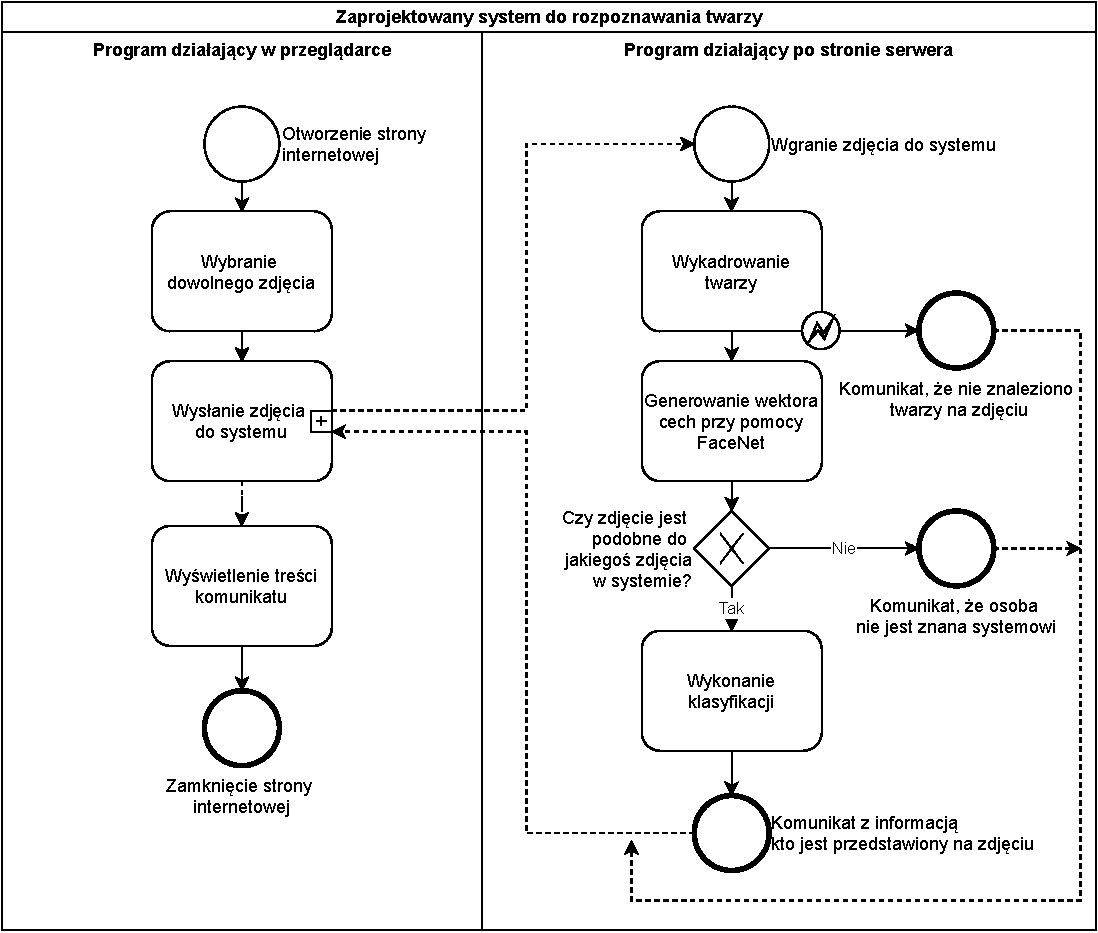
\includegraphics[width=1\textwidth]{images/schemat_blokowy_systemu}
    \caption{Schemat blokowy zaprojektowanego systemu}
    \customsource
    \label{fig:schemat_blokowy_systemu}
\end{figure}
    \chapter{Wybór technologii oraz narzędzi}


\section{Wykrywanie twarzy na zdjęciu}

Wykrywanie twarzy to pierwszy krok w zaprojektowanym systemie.
Z powodu, że jest on umieszczony na samym początku, proces ten musi być maksymalnie skuteczny.
Jeżeli na zdjęciu nie zostanie wykryta twarz, to cały proces zakończy się z negatywnym rezultatem.
\textbf{Twarzy nie będzie można zidentyfikować, jeżeli nie zostanie ona znaleziona.}
Oznacza to, że twarze muszą być wykrywane z różnymi orientacjami, kątami,
poziomem oświetlenia, makijażem, kapeluszami, zarostem, fryzurami, okularami, wiekiem i tak dalej.
Niestety twarz ludzka jest obiektem dynamicznym i ma duży stopień zmienności w wyglądzie,
co sprawia, że wykrywanie twarzy jest trudnym problemem w widzeniu komputerowym~\cite{HJELMAS2001236}.

W artykule z 2016 roku zatytułowanym
``Joint Face Detection and Alignment Using Multitask Cascaded Convolutional Networks''~\cite{zhang2016joint}
została zaproponowana wielozadaniowa kaskadowa konwolucyjna sieć neuronowa
(MTCNN\footnote{Skrót z języka angielskiego od Multi-Task Cascaded Convolutional Neural Networks })
do wykrywania twarzy.
Sieć ta zyskała duża popularność, ponieważ osiągnęła wówczas najlepszy wyniki
w wykrywaniu twarzy na zdjęciach dla wybranych zbiorów danych.
Kolejną zaletą zaproponowanej sieci neuronowej jest to, że jest w stanie
rozpoznać punkty orientacyjne twarzy, takie jak oczy, usta i nos.
Wyniki przeprowadzonych eksperymentów w artykule zostały przedstawione na rysunku~\ref{fig:mtcnn_wyniki}.

\begin{figure}[P]
    \centering
    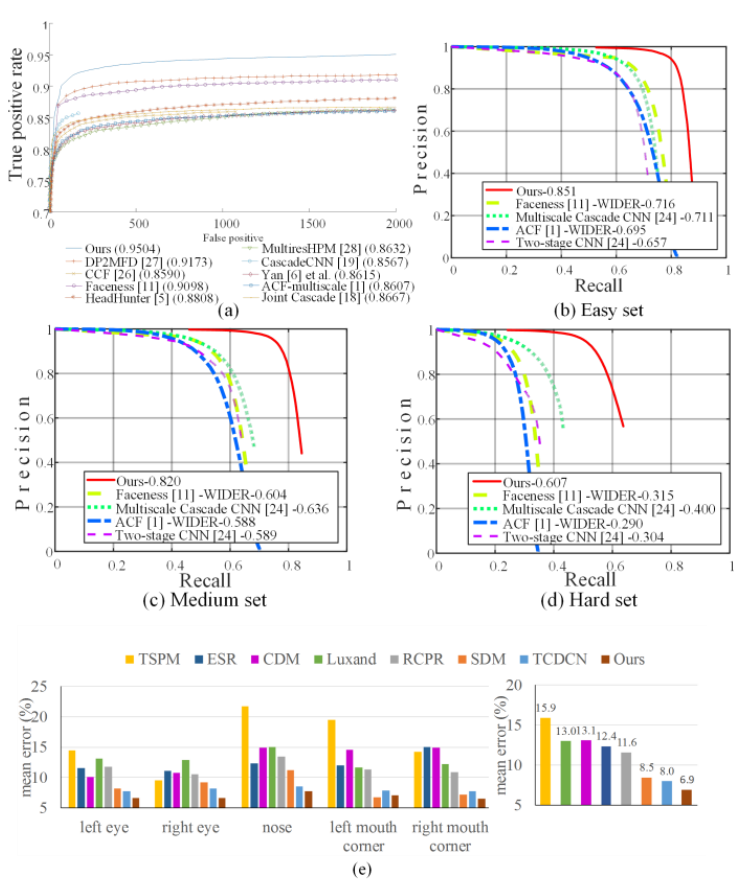
\includegraphics[width=1\textwidth]{images/mtcnn-wyniki}
    \caption{
        Wyniki przeprowadzonych eksperymentów. Słowo ``Ours'' oznacza sieć MTCNN.
        (a) wyniki z testów na bazie FDDB.
        (b-d) wyniki z testów dla trzech kolejnych zbiorów na bazy Wider Face.
        (e) Wyniki z testów dla wyrównania twarzy na bazie AFLW.
    }
    \bibsource{\cite{zhang2016joint}}
    \label{fig:mtcnn_wyniki}
\end{figure}


W internecie znajduje się spora liczba implementacji MTCNN~\cite{mtznn_all_impls}.
Spośród dostępnych została wybrana sieć napisana przez \textit{Iván de Paz Centeno}
i udostępniona na portalu GitHub\footnote{GitHub - dostawcą platformy internetowej do tworzenia
oprogramowania i kontroli wersji za pomocą narzędzia Git udostępniania
pod adresem \url{https://github.com}. } (\url{https://github.com/ipazc/mtcnn}) na zasadach licencji MIT\footnote{Licencja MIT daje użytkownikom
nieograniczone prawo do używania, kopiowania, modyfikowania i rozpowszechniania (w tym sprzedaży)
    oryginalnego lub zmodyfikowanego programu w postaci binarnej lub źródłowej.
    Jedynym wymaganiem jest, by we wszystkich wersjach zachowano warunki licencyjne i informacje o autorze.
}~\cite{ipazc/mtcnn}.
Główną zaletą wybranej implementacji jest łatwość użycia.
Sieć została napisana w języku programowania python w bibliotece TensorFlow
i całość udostępniona jako pakiet z możliwością instalacji
przez PIP\footnote{PIP - narzędzie do instalowania pakietów python}.


\section{FaceNet}

FaceNet to architektura, oparta na głębokiej sieci neuronowej, która bezpośrednio uczy się mapowania
z obrazów twarzy do zwartej przestrzeni euklidesowej,
w której odległości bezpośrednio odpowiadają mierze podobieństwa twarzy~\cite{schroff2015facenet}.
Wynikiem działania sieci jest wektor składający się z elementów charakteryzujący daną twarz.
Długość wektora jest zależna od konkretnej implementacji.
Po utworzeniu przestrzeni euklidesowej na bazie dostępnych zdjęć twarzy,
zadania polegające na identyfikacji, weryfikacji czy grupowaniu
sprowadzają się do pomiaru odległości pomiędzy poszczególnymi wektorami cech~\cite{schroff2015facenet}.
Wizualizacja procesu mapowania zdjęcia do przestrzeni
euklidesowej została przedstawiona na rysunku~\ref{fig:facenet_zastosowanie}.

\begin{figure}[]
    \centering
    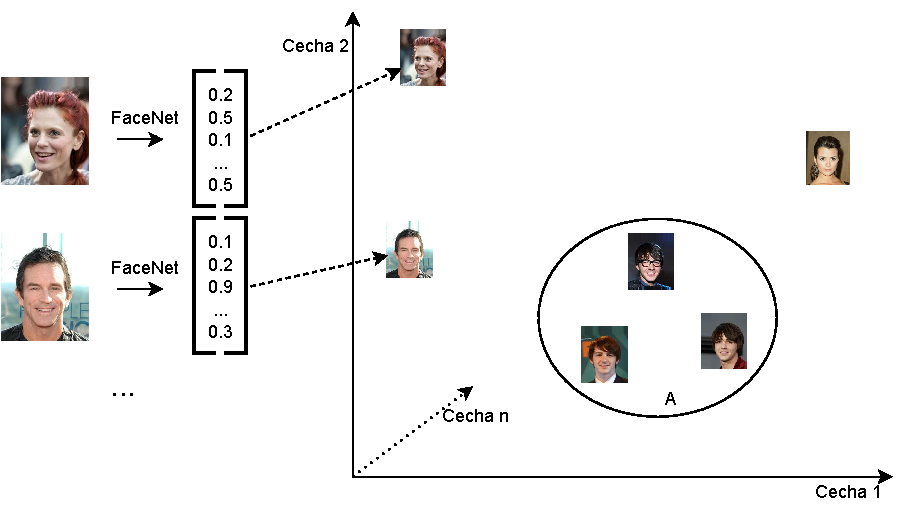
\includegraphics[width=1\textwidth]{images/facenet_euc}
    \caption{
        Proces umieszczania wektorów cech w przestrzeni euklidesowej.
        Zdjęcia przedstawiające tę samą osobę znajdą się bliżej siebie względem zdjęć innych osób.
        Literą ``A'' zostały oznaczone zdjęcia przedstawiające tę samą osobę.
    }
    \customsource
    \label{fig:facenet_zastosowanie}
\end{figure}

\subsection{Zasada działania}

FaceNet pobiera obraz twarzy osoby jako dane wejściowe i wyprowadza wektor,
który reprezentuje najważniejsze cechy twarzy (wektor cech).
Operacje ta, jest pewnego rodzaju kompresją, której zadaniem jest zmniejszenie ilości informacji
na temat danej rzeczy (w tym wypadku zdjęcia twarzy) bez utraty kluczowych informacji.
Informacje, jakie są pobierane ze zdjęcia, nie są z góry zdefiniowane.
Za odpowiedni dobór parametrów jest odpowiedzialna głęboka sieć neuronowa, która traktowana jest
jako czarna skrzynka, czyli miejsce, gdzie znane są tylko dane wejściowe oraz dane wyjściowe.
Oznacza to, że nie są znane parametry, które są pobierane ze zdjęcia,
a wartości w wektorze cech generowane na wyjściu są trudne, o ile w ogóle możliwe do zinterpretowania.

Oprócz samej sieci neuronowej FaceNet składa się również z innych warstw: normalizacji L2 oraz
funkcji strat \textit{triplet loss} (rysunek~\ref{fig:facenet_arch}).
Normalizacja L2 polega na takim zmodyfikowaniu wartości otrzymanego zbioru, aby w każdym wierszu
suma kwadratów była zawsze równa $1$,
natomiast zadaniem funkcji \textit{triplet loss} jest, w procesie trenowania sieci,
minimalizowanie odległości pomiędzy prawdziwymi
wyrażeniami oraz maksymalizowanie dla fałszywych~\cite{chechik2010large}.
Innymi słowy, celem jest, aby odległości między wektorami tych samych osób były jak najmniejsze,
a odległości pomiędzy wektorami różnych osób --- maksymalne.
Wzór matematyczny został przedstawiony równaniem~\ref{eq:triplet_loss},
natomiast zasada działania w sposób graficzny przedstawiona na rysunku~\ref{fig:triplet_loss}.


\begin{equation}
    L = \sum_{i}^{N} [  \| f(x_i^a) - f(x_i^p) \| ^2_2 - \| f(x_i^a) - f(x_i^n) \| ^2_2 + \alpha ] _+
    \label{eq:triplet_loss}
\end{equation}

gdzie:

$x_i^a$ - wektor zdjęcia wzorcowego

$x_i^p$ - wektor zdjęcia ``prawdziwego'' względem wzorca

$x_i^n$ - wektor zdjęcia ``fałszywego'' względem wzorca

$\alpha$ - margines odległości pomiędzy wektorami

\pagebreak

\begin{figure}[]
    \centering
    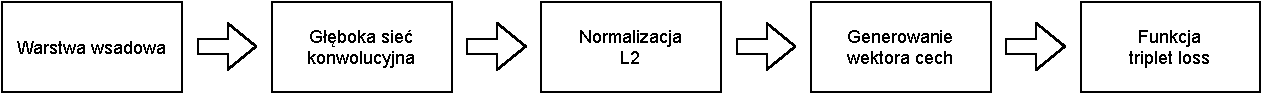
\includegraphics[width=1\textwidth]{images/facenet_arch}
    \caption{ Architektura FaceNet z podziałem na poszczególne warstwy }
    \customsource
    \label{fig:facenet_arch}
\end{figure}

\begin{figure}[]
    \centering
    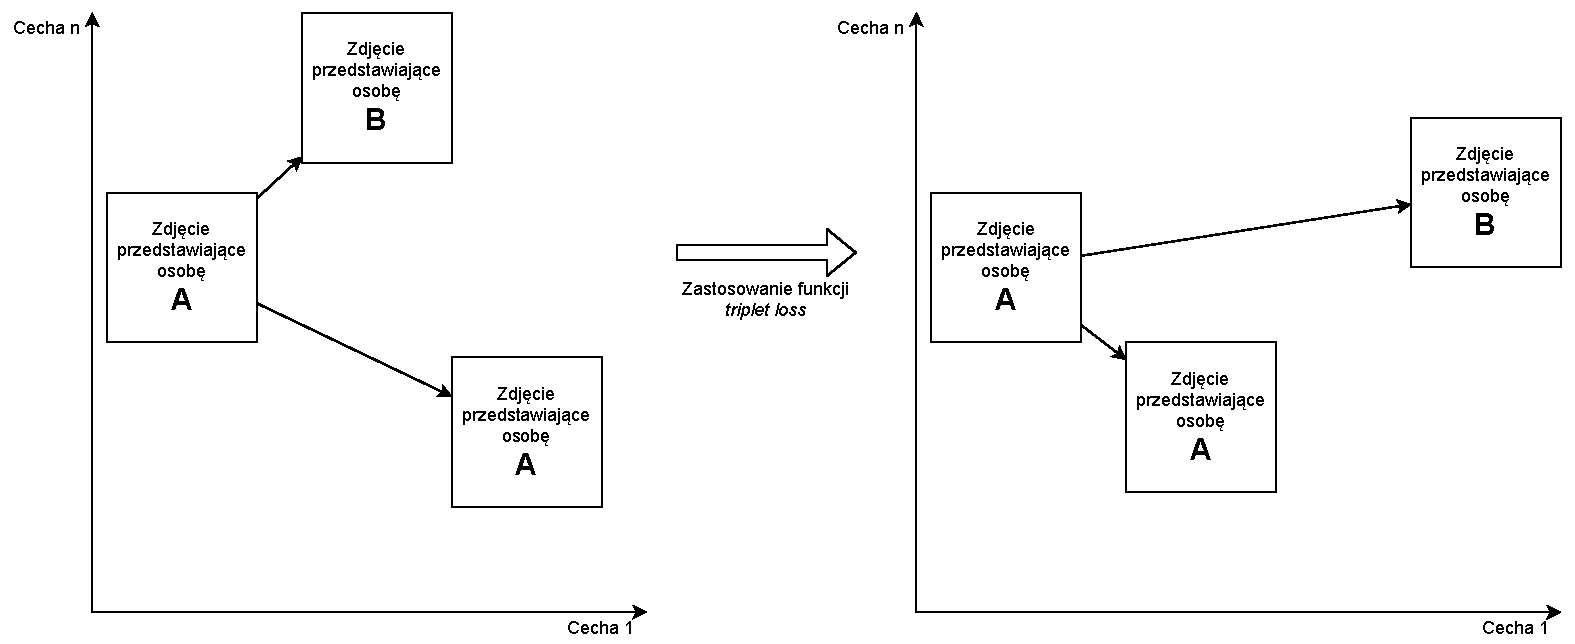
\includegraphics[width=1\textwidth]{images/triplet_loss}
    \caption{ Uproszczony schemat obrazujący zasadę działania funkcji strat \textit{triplet loss} }
    \customsource
    \label{fig:triplet_loss}
\end{figure}


Całość procesu uczenia się sieci FaceNet, można w uproszczeniu podsumować w następujących krokach:

\begin{enumerate}
    \item zdefiniowanie parametrów początkowych sieci,
    \item wygenerowanie wektorów cech twarzy,
    \item użycie funkcji strat \textit{triplet loss},
    \item dostosowanie się parametrów sieci tak, aby przykład pozytywny był bliżej zdjęcia wzorcowego, niż przykład negatywny,
    \item powrót do kroku drugiego tak długo, aż zwracane wektory osiągną zadaną dokładność
\end{enumerate}

\subsection{Wpływ wielkości zdjęcia na działanie sieci}

W pracy pod tytułem \textit{Facenet: A unified embedding for face recognition and clustering}~\cite{schroff2015facenet}
została wytrenowana sieć o architekturze FaceNet na zdjęciach w formacie JPEG o rozmiarach 220 na 220 pikseli.
Podczas testowania wytrenowanej sieci, po dostarczeniu zdjęć o mniejszych rozmiarach (względem rozmiarów
zdjęć, na których sieć była trenowana) okazało się, że sieć ta jest również bardzo skuteczna.
Sieć miała akceptowalną skuteczność nawet po dostarczeniu zdjęć o rozmiarach 80 na 80 pikseli.
Trenowanie sieci na zdjęciach o mniejszej rozdzielczości mogłoby jeszcze poprawić ten wynik.
Dokładne informacje na temat wpływu liczby pikseli na
trafność sieci zostały przedstawione w tabeli~\ref{tab:quality_pixels_to_rate}

\begin{table}[]
    \caption{Wpływ jakości zdjęcia oraz liczby pikseli na trafność sieci FaceNet. Źródło: \cite{schroff2015facenet}}
    \label{tab:quality_pixels_to_rate}
    \begin{minipage}{.5\linewidth}
        \centering
        \begin{tabular}{|l|l|}
            \hline
            Liczba pikseli                & Trafność \\ \hline
            1 600 \hspace{15px} (40x40)   & 37.8\%   \\ \hline
            6 400 \hspace{15px}     (80x80)    & 79.5\%   \\ \hline
            14 400 \hspace{10px}  (120x120) & 84.5\%   \\ \hline
            25 600 \hspace{10px}  (160x160) & 85.7\%   \\ \hline
            65 536 \hspace{10px}  (256x256) & 86.4\%   \\ \hline
        \end{tabular}
    \end{minipage}%
    \begin{minipage}{.5\linewidth}
        \centering
        \begin{tabular}{|l|l|}
            \hline
            Jakość JPEG & Trafność \\ \hline
            10          & 67.3\%   \\ \hline
            20          & 81.4\%   \\ \hline
            30          & 83.9\%   \\ \hline
            50          & 85.5\%   \\ \hline
            70          & 86.1\%   \\ \hline
            90          & 86.5\%   \\ \hline
        \end{tabular}
    \end{minipage}
\end{table}

\subsection{Użycie wytrenowanej sieci}

W projektowanym systemie zostanie użyty wytrenowany model \textit{Keras FaceNet}~\cite{taniai-2018},
który został wyszkolony na bazie zdjęć dostarczonych przez MS-Celeb-1M~\cite{microsoft-2020-celeb1m}
i udostępniony przez \textit{Hiroki Taniai}~\cite{taniai-no-date}.
Dostarczane zdjęcia twarzy powinny być kolorowe, w formacie RGB oraz
o rozmiarach 160 pikseli na 160 pikseli~\cite{brownlee-2019}.


\section{Kadrowanie i standaryzacja}

Do przetwarzania plików graficznych zostanie wykorzystana biblioteka \textit{PILLOW} napisana w języku python.
Biblioteka wspiera wiele formatów graficznych,
w tym te najpopularniejsze jak \textit{PNG}, \textit{GIF}, \textit{JPEG} oraz \textif{BMP}~\cite{pillow_doc},
dzięki czemu nie będzie wymagane, aby użytkownik sam konwertował plików graficznych do odpowiedniego formatu.
Biblioteka \textit{PILLOW} zostanie również wykorzystana do wycinania zdjęcia twarzy oraz standaryzacji
i normalizacji już wykadrowanego zdjęcia.


\section{Klasyfikacja}

Ostatnim krokiem w systemie jest dokonanie klasyfikacji wygenerowanego wektora cech,
czyli określenie, do jakiej grupy należy wektor na podstawie próbek uczących.
Innymi słowy, etap ten polega na zwróceniu informacji, do kogo najbardziej pasuje przesłane zdjęcie,
opierając się na fotografiach dostępnych w systemie.

Jednym z szeroko stosowanych algorytmów klasyfikacji jest
\textbf{maszyna wektorów nośnych} (ang. support vector machine — SVM).
Klasyfikator ten konstruuje hiperpłaszczyznę lub ich zbiór w przestrzeni wielowymiarowej,
na podstawie otrzymanych próbek, która oddziela poszczególne klasy.
Optymalizowanie modelu SVM polega na maksymalizacji marginesu pomiędzy płaszczyzną a poszczególnymi klasami,
ponieważ na ogół nim większy margines, tym mniejszy jest błąd generalizacji~\cite{hastie2009elements}.
Koncepcja klasyfikatora została zaprezentowana na rysunku~\ref{fig:svm}.


\begin{figure}[]
    \centering
    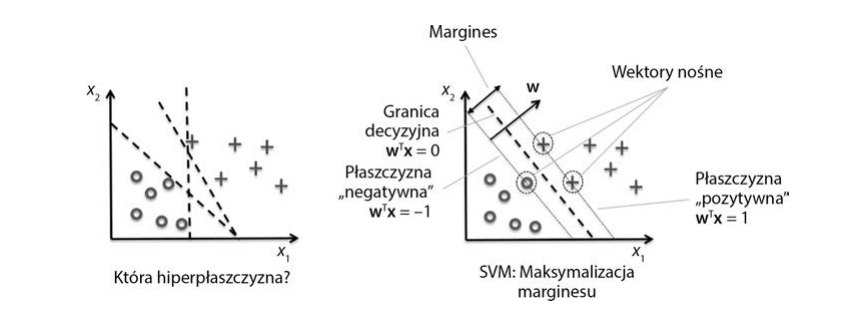
\includegraphics[width=1\textwidth]{images/smv}
    \caption{
        Model maszyny wektorów nośnych.
        Po lewej możliwe położenia hiperpłaszczyzny, po prawej zoptymalizowany model wraz z objaśnieniami.
    }
    \bibsource{\cite{raschka2017python}}
    \label{fig:svm}
\end{figure}

Jeśli dane uczące są liniowo separowalne, to można wybrać dwie równoległe hiperpłaszczyzny,
które oddzielają dwie klasy danych, tak aby odległość między nimi była maksymalna.
Obszar ograniczony przez te dwie hiperpłaszczyzny nazywany jest ``marginesem'',
a hiperpłaszczyzna maksymalnego marginesu to hiperpłaszczyzna leżąca w połowie odległości między nimi.
Problem optymalizacji algorytmu został przedstawiony równaniem~\ref{eq:hard_margin}.
Lewą stroną tego równania jest odległość pomiędzy hiperpłaszczyzną ``pozytywną'' a ``negatywną'',
zatem, w celu maksymalizacji marginesu, należy zmaksymalizować $\frac{2}{||w||}$ lub
minimalizować odwrotność wyrażenia, czyli $\frac{1}{2}||w||^2$.

\begin{equation}
    \begin{aligned}
        & \frac{ w^T (x_{poz} - x_{neg}) }{ ||w|| } = \frac{2}{||w||} \\
        \text{gdzie:} \\
        w & \text{ - wektor normalny do granicy decyzyjności}
        \\
        x_{poz} & \text{ - ``pozytywny'' wektor nośny}
        \\
        x_{neg} & \text{ - ``negatywny'' wektor nośny}
    \end{aligned}
    \label{eq:hard_margin}
\end{equation}
\bigskip

W przypadku danych liniowo separowalnych równanie~\ref{eq:hard_margin} musi
spełniać warunki przedstawione w równaniu~\ref{eq:hard_margin_class}.
Równania te oznaczają, że wszystkie negatywne próbki powinny wylądować po stronie
negatywnej hiperpłaszczyzny, a wszystkie próbki pozytywne po stronie hiperpłaszczyzny pozytywnej.

\begin{equation}
    \begin{aligned}
        w_0 +w^{T}x^{(i)} &\geq 1 && \text{ jeśli } y^{(i)} =1
        \\
        w_0 +w^{T}x^{(i)} &\leq -1 && \text{ jeśli } y^{(i)} =-1
        \\
        \text{dla } i&= 1\dots N
        \\
        \text{ gdzie: } \\
        N & \text{  - liczba próbek}
        \\
        w_0 +w^{T}x^{(i)} & \text{  - odległość od granicy decyzyjności}
    \end{aligned}
    \label{eq:hard_margin_class}
\end{equation}

\bigskip

W przypadku, gdy dane nie są liniowo separowalne (rysunek~\ref{fig:sofm_margin}) wprowadza się dodatkową zmienną $\xi$.
Motywacją wprowadzenia tej zmiennej jest potrzeba ``uelastycznienia'' liniowych
ograniczeń (równanie~\ref{eq:hard_margin_class}) podczas analizowania nieliniowo rozdzielnych danych,
co pozwala na uzyskanie zbieżności algorytmu uczącego w obecności nieprawidłowych klasyfikacji
podczas stosowania odpowiedniej funkcji strat.

\begin{figure}[]
    \centering
    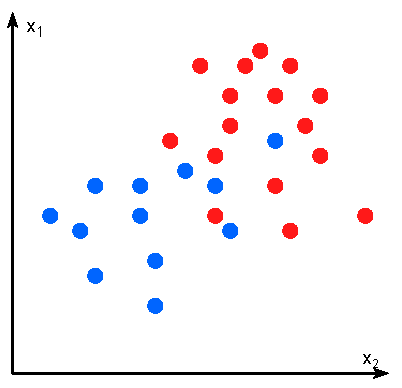
\includegraphics[width=0.3\textwidth]{images/soft-margin.drawio}
    \caption{ Przykład nieliniowo rozdzielnych próbek}
    \customsource
    \label{fig:sofm_margin}
\end{figure}

Po wprowadzeniu zmiennej $\xi$ do równiania~\ref{eq:hard_margin_class},
równanie to przybiera postać opisaną wzorami~\ref{eq:soft_margin}.

\begin{equation}
    \begin{aligned}
        w_0 +w^{T}x^{(i)} &\geq 1 - \xi^{(i)} && \text{ jeśli } y^{(i)} =1
        \\
        w_0 +w^{T}x^{(i)} &\leq -1 + \xi^{(i)} && \text{ jeśli } y^{(i)} =-1
        \\
        \text{dla } i&= 1\dots N \\
        \text{gdzie:} \\
        \xi & \text{ - wartość przesunięcia granicy przynależności}
    \end{aligned}
    \label{eq:soft_margin}
\end{equation}

Nowym celem optymalizacji staje wtedy się równanie~\ref{eq:hard_svm_min_problem}.
Za pomocą zmiennej $C$ kontroluje się wagę kary za niewłaściwą klasyfikację.
Duża wartość parametru $C$ odpowiada wysokim karom za błędy, z kolei przy niskich wartościach
kara nie będzie mocno wpływać na szerokość marginesu.
Dzięki temu parametrowi jest się w stanie regulować kompromis pomiędzy
obciążeniem a wariancją~\cite{raschka2017python} (rysunek~\ref{fig:wplyw_c_na_svm}).

\begin{equation}
    \begin{aligned}
        &\frac{1}{2}||w||^2 + C (\sum_{i}^{N} \xi^{(i)})\\
        \text{gdzie:} \\
        &C \text{ - mnożnik kary za złą klasyfikację}
    \end{aligned}
    \label{eq:hard_svm_min_problem}
\end{equation}

\begin{figure}[]
    \centering
    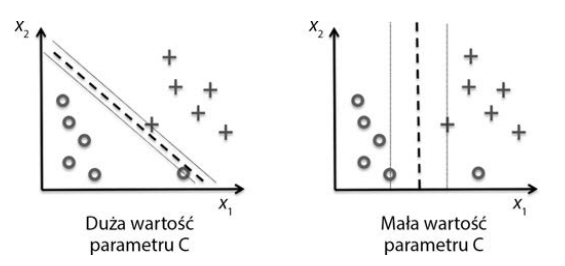
\includegraphics[width=0.7\textwidth]{images/wplyw_c_na_svm}
    \caption{  Wpływ zmiennej C na szerokość marginesu }
    \bibsource{\cite{raschka2017python}}
    \label{fig:wplyw_c_na_svm}
\end{figure}

\bigskip

W przypadku, gdy dostarczone dane nie są separowalne za pomocą hiperpłaszczyzny
w $N$ wymiarach (rysunek~\ref{fig:dane_nie_separowalne_liniowo})
wprowadza się dodatkowe wymiary za pomocą funkcji mapującej $\phi$.
Dodatkowe wymiary wprowadza się tak długo, aż dane staną się liniowo separowalne.
Przykładowo, w celu wyznaczenia granicy decyzyjności danych
przedstawionych na rysunku~\ref{fig:dane_nie_separowalne_liniowo},
funkcja mapująca, za pomocą której będzie możliwe wyznaczenie hiperpłaszczyzny,
została przedstawiona równaniem~\ref{eq:przykladowy_kernel}.
Rezultat mapowania danych z rysunku~\ref{fig:dane_nie_separowalne_liniowo} przez funkcję~\ref{eq:przykladowy_kernel}
został przedstawiony na rysunku~\ref{fig:wyniki_mapowan}.
Po wykonaniu mapowania oraz wyznaczeniu hiperpłaszczyzny dokonuje się rzutowania do pierwotnej przestrzeni cech ($\phi^{-1}$).

\begin{equation}
    \begin{aligned}
        \phi(x_1, x_2) = (z_1, z_2, z_3) = (x_1, x_2, x_1^2 + x_2^2)
    \end{aligned}
    \label{eq:przykladowy_kernel}
\end{equation}

\begin{figure}[]
    \centering
    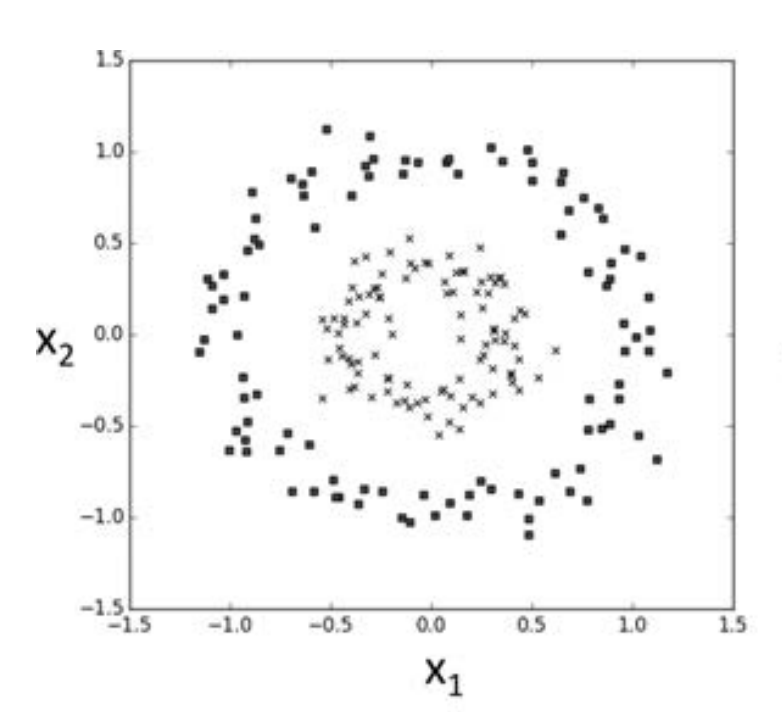
\includegraphics[width=0.5\textwidth]{images/dane_nie_separowalne_liniowo}
    \caption{  Zestaw danych nie separowalnych liniowo }
    \bibsource{\cite{raschka2017python}}
    \label{fig:dane_nie_separowalne_liniowo}
\end{figure}

\begin{figure}[]
    \centering
    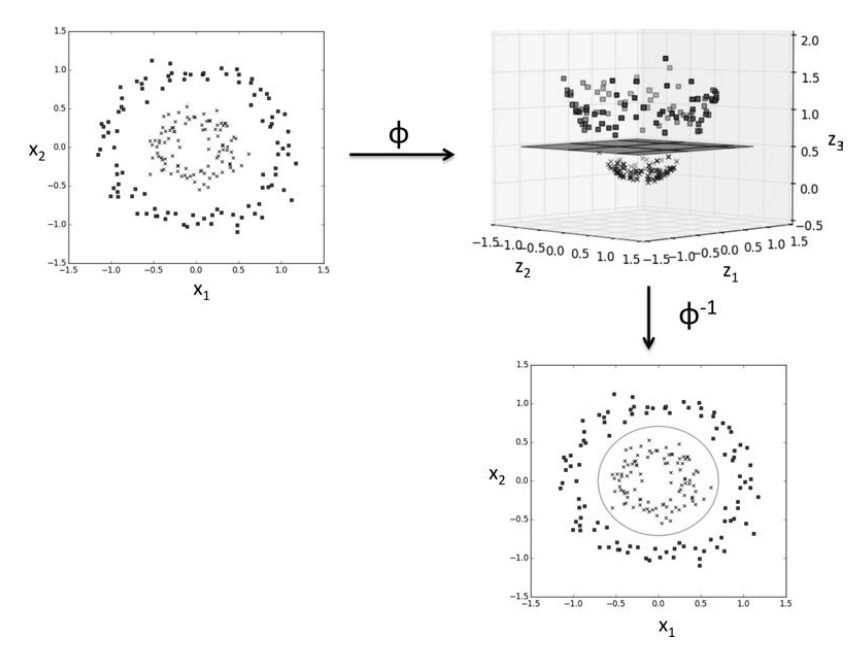
\includegraphics[width=0.5\textwidth]{images/wyniki_mapowan}
    \caption{ Sposób wyznaczania nieliniowej granicy decyzyjności }
    \bibsource{\cite{raschka2017python}}
    \label{fig:wyniki_mapowan}
\end{figure}

\bigskip

Wszystkie opisane wyżej przypadki dotyczą problemów binarnych,
czyli takich gdzie dostarczona próbka należy do jednej z dwóch klas.
W związku z tym, że SVM obsługuje tylko klasyfikację binarną, dlatego w przypadku
gdy dana próbka może należeć do jeden z $N$ klas (klasyfikacja wieloklasowa)
dokonuje się rozbicia jednego problemu klasyfikacji wieloklasowej na wiele problemów klasyfikacji binarnej.
W tym celu stosuje się jedną z dwóch strategii - jeden kontra jeden (ang. one vs one --- OvO)
lub jeden przeciwko wszystkim (ang. one vs all --- OvA).
Obie te strategie zostały przedstawione na rysunku~\ref{fig:ovr} oraz~\ref{fig:ovo}.


\begin{figure}[]
    \centering
    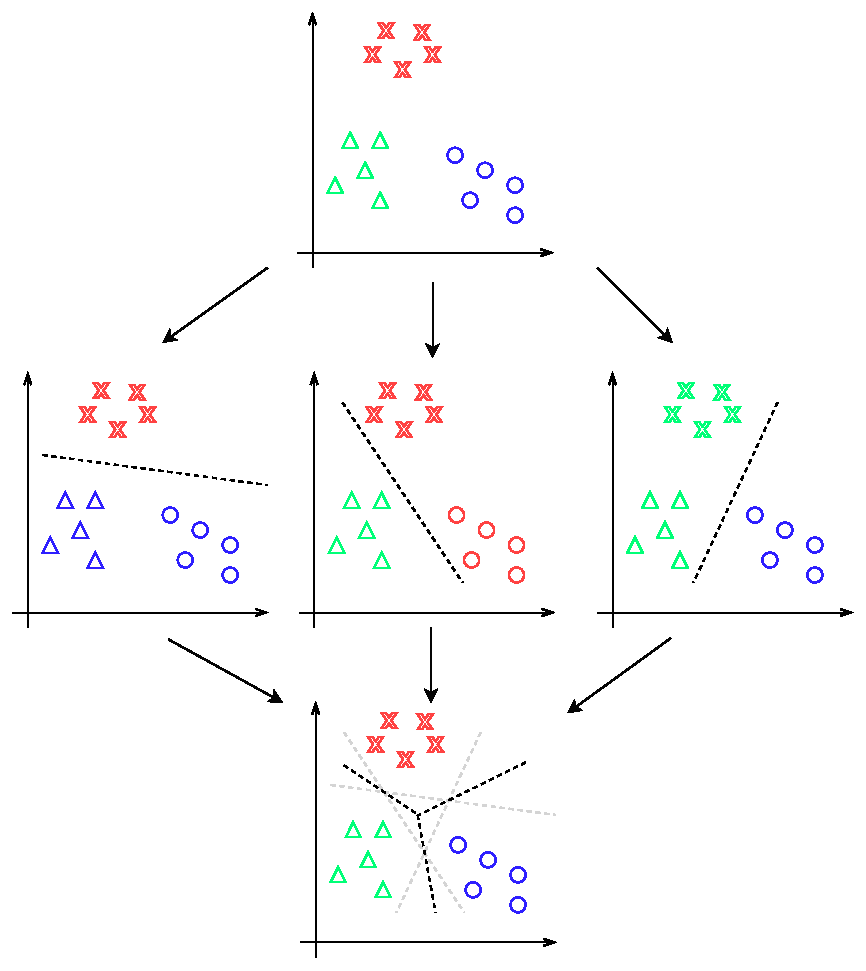
\includegraphics[width=0.7\textwidth]{images/ovr}
    \caption{ Strategia jeden przeciwko wszystkim }
    \customsource
    \label{fig:ovr}
\end{figure}

\begin{figure}[]
    \centering
    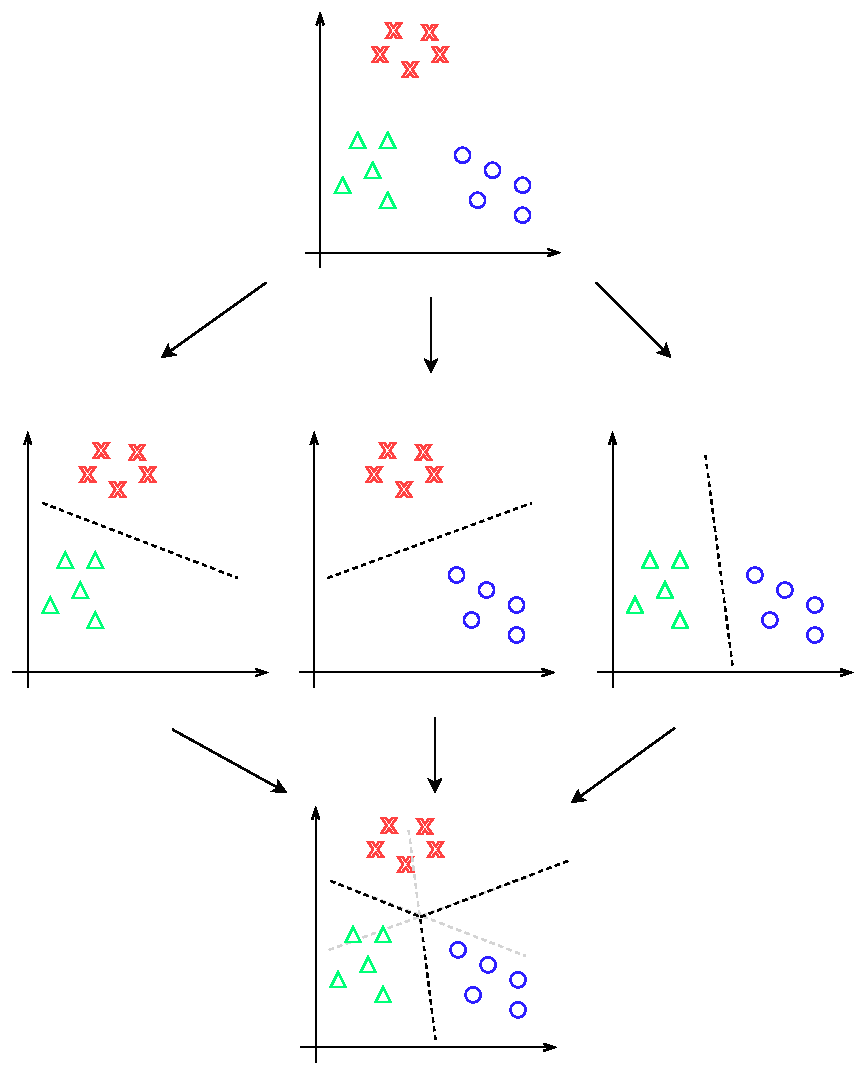
\includegraphics[width=0.7\textwidth]{images/ovo}
    \caption{ Strategia jeden kontra jeden }
    \customsource
    \label{fig:ovo}
\end{figure}



\section{Obsługa systemu}

Całość zaprojektowanego systemu ma być dostępna z przeglądarki internetowej.
Aby sprostać temu wymaganiu, należy napisać usługę, która jest w stanie obsługiwać połączenia
HTTP\footnote{Skrót z języka angielskiego od słów Hypertext Transfer Protocol}.
Z powodu, że narzędzia do wykrywania twarzy, obróbki zdjęć oraz FaceNet są udostępnione w języku python,
program zostanie również napisany w tym języku.
Oprócz samej strony internetowej potrzebna jest również baza danych,
w której będą przechowywane informacje o dostępnych zdjęciach.
Same zdjęcia będą przechowywane na serwerze plików.
Sporym ułatwieniem będzie również panel umożliwiający zarządzanie dostępnymi zdjęciami w systemie.

Narzędziem, które spełni wyżej postawione wymagania jest platforma programistyczna \textit{Django},
która umożliwia w łatwy sposób zarządzanie bazą danych za pomocą mapowania obiektowo-relacyjnego,
pozwala na zarządzanie danymi dostępnymi w bazie danych poprzez panel administratora, dostępny
z poziomu przeglądarki oraz co najważniejsze, jest napisana w języku python~\cite{djangodoc}.
    \chapter{Implementacja systemu}


\section{Kadrowanie twarzy}

Zdjęcia, które zostaną przesłane na serwer, należy w pierwszej kolejności odpowiednio przygotować.
W tym celu została wykorzystana wcześniej wspomniana biblioteka PILLOW,
która ma za zadanie wykonać przekształcenie otrzymanego pliku do tablicy pikseli.
Otrzymana tablica następnie trafia do sieci MTCNN, która zwraca informacje na temat wykrytych twarzy,
po czym następuje wycinanie fragmentu zdjęcia przedstawiającego samą twarz.
Jeżeli nie zostaną znalezione żadne twarze, funkcja rzuci odpowiednim błędem.


\section{Generowanie wektora cech}

Po wykadrowaniu twarzy, kolejnym krokiem jest wygenerowanie wektora cech.
Odpowiednio przygotowana wcześniej tablica pikseli jest standaryzowana,
ponieważ wymaga tego używana implementacja architektury FaceNet, a następnie wykonywana jest predykcja.
Jako wynik działa funkcji zwracany jest opisany wcześniej wektor cech.


\pagebreak


\section{Ocena podobieństwa twarzy}

FaceNet został nauczony tak, aby mapować zdjęcia twarzy do zwartej przestrzeni euklidesowej,
w której odległości pomiędzy punktami bezpośrednio odpowiadają mierze podobieństwa twarzy.
Oznacza to, że jeżeli odległość pomiędzy dwoma punktami w przestrzeni
jest względnie mała, to jest wysoce prawdopodobne, że zdjęcia twarzy przedstawiają tę samą osobę.
Mając to na uwadze, można znaleźć odległość, poniżej której zostałoby uznane, że zdjęcia
przedstawiają tę samą osobę (rysunek~\ref{fig:szukanie_progu}).

\begin{figure}[H]
    \centering
    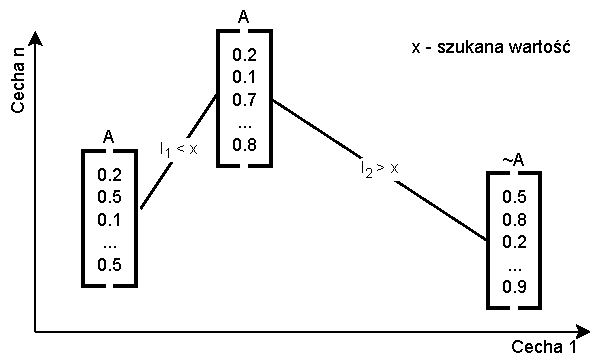
\includegraphics[width=1\textwidth]{./images/szukanie_progu}
    \caption{ Wizualizacja szukanego progu podobieństwa. Jeżeli odległość pomiędzy punktami jest
    zmniejsza niż wartość ``x'' to program powinien uznać, że wektory opisują tę samą osobę. }
    \customsource
    \label{fig:szukanie_progu}
\end{figure}

\pagebreak

\subsection{Poszukiwanie odległości}

Do poszukiwania wartości progu zostało wykorzystanych około \num{5000} losowo wybranych zdjęć,
przedstawiających około \num{500} różnych osób, po około \num{10} zdjęć na osobę,
z bazy CelebA~\cite{liu2015faceattributes}.
Na każdym zdjęciu zostało następnie wykonane kadrowanie twarzy oraz generowanie wektora cech.
Ostatnim elementem było zbadanie odległości pomiędzy wszystkimi wektorami tych samych oraz różnych osób.
Całość badania można podsumować w następujących krokach:
\begin{enumerate}
    \item wygenerowania wektora cech dla każdego z dostępnych zdjęć,
    \item wybranie wektora cech ze zbioru,
    \item zmierzenie odległości pomiędzy wybranym wektorem i wszystkimi pozostałymi wektorami z uwzględnieniem,
    czy wektory cech reprezentują tę samą osobę, czy dwie różne osoby,
    \item powrót do kroku drugiego do momentu, aż zostaną zbadane wszystkie odgległości (każdy z każdym).
\end{enumerate}
Wyniki przeprowadzonych kroków zostały przedstawione w postaci histogramów na rysunku~\ref{fig:porownanie_histogramow_odleglosci}.

\begin{figure}[H]
    \centering
    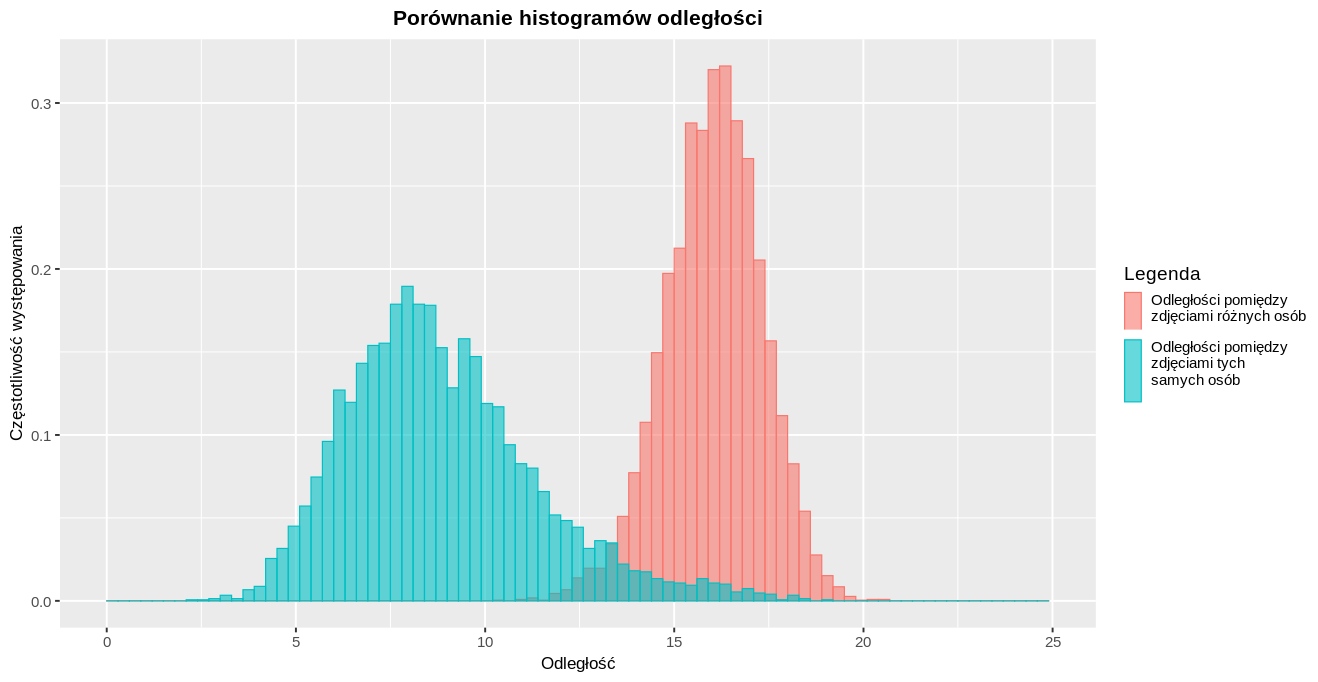
\includegraphics[width=1\textwidth]{./images/porownanie_histogramow_odleglosci}
    \caption{ Porównanie histogramów odległości pomiędzy wektorami twarzy tych samych oraz różnych osób }
    \customsource
    \label{fig:porownanie_histogramow_odleglosci}
\end{figure}

\pagebreak

Na podstawie histogramów (rysunek~\ref{fig:porownanie_histogramow_odleglosci}) można zauważyć,
że nie istnieje taka wartość, która jest w stanie odseparować przedstawione zbiory.
Należy jednak zwrócić uwagę na to, że w badaniu zostały wzięte odległości pomiędzy \textbf{każdym} zdjęciem z grupy.
Przy ocenie podobieństwa pomiędzy twarzami nie ma potrzeby patrzenia na odległości na całym zbiorze zdjęć.
Po wygenerowaniu wektora cech dla danego zdjęcia interesujący jest tylko ten wektor, który
leży \textbf{najbliżej} wygenerowanego (rysunek~\ref{fig:najmniejsze}).

\begin{figure}[H]
    \centering
    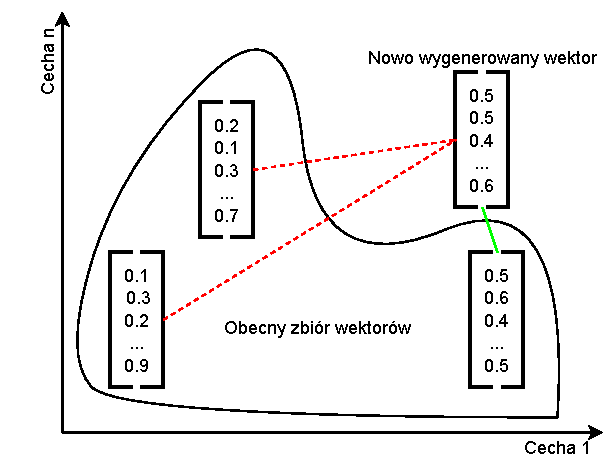
\includegraphics[width=1\textwidth]{./images/dlaczego_najmniejsze}
    \caption{ Schemat obrazujący najbliższą odległość pomiędzy nowym wektorem a zbiorem.
    Na czerwono zostały oznaczone odległości do dalszych wektorów. Na zielono została oznaczona odległość
    do najbliższego wektora i to względem niego system powinien oceniać podobieństwo.
    }
    \customsource
    \label{fig:najmniejsze}
\end{figure}

\pagebreak

Biorą pod uwagę opisany problem, wyżej opisane badanie zostało powtórzone, jednak w tym przypadku
zostały zapisane tylko odległość do najbliższego wektora.
Całość zatem można podsumować w następujących krokach:
\begin{enumerate}
    \item wygenerowania wektora cech dla każdego z dostępnych zdjęć,
    \item wybranie wektora cech ze zbioru,
    \item znalezienie wektora, który leży najbliżej względem wybranego i zapisanie odległości
    z uwzględnieniem czy znaleziony wektor reprezentuje tę samą osobę,
    \item powrót do kroku drugiego do momentu, aż zostaną wybrane wszystkie wektory.
\end{enumerate}
Wyniki powtórzonego badania zostały ponownie przedstawione w postaci
histogramów na rysunku~\ref{fig:wykres_najmniejszych_odleglosc_wspolny}.

\begin{figure}[H]
    \centering
    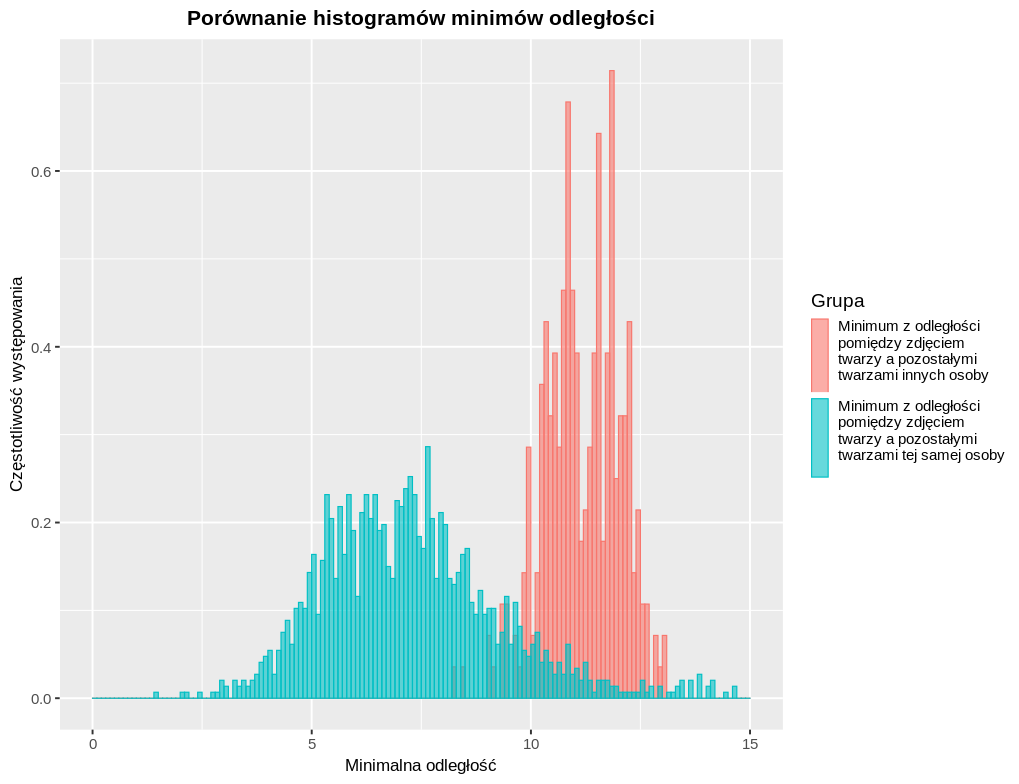
\includegraphics[width=1\textwidth]{images/wykres_najmniejszych_odleglosc_wspolny}
    \caption{
        Porównanie histogramów najmniejszych odległości pomiędzy
        zdjęciami twarzy tych samych oraz różnych osób.
    }
    \customsource
    \label{fig:wykres_najmniejszych_odleglosc_wspolny}
\end{figure}

\pagebreak

Z histogramów (rysunek~\ref{fig:wykres_najmniejszych_odleglosc_wspolny}) wykonanego badania również wynika,
że nie istnieje taka wartość, która będzie w stanie odseparować przedstawione zbiory.
Konsekwencją tego jest, że dla dowolnego ``x'' będą istnieć przypadki, dla których
zdjęcia błędnie zostaną uznane, że przedstawiają tę samą osobę.
Należy zatem znaleźć taką wartość ``x'', dla której funkcja oceniająca, czy wektory
dotyczą tej samej osoby, będzie miała największą skuteczność.
Przedział, w jakim należy spodziewać się największej trafności,
powinien (jak wynika z rysunku~\ref{fig:wykres_najmniejszych_odleglosc_wspolny})
znaleźć się w przedziale od \num{8} do \num{12}, ponieważ na tym odcinku
oba histogramy pokrywają się na największym obszarze.

\subsection{Odległość o największej skuteczności}

W celu sprawdzania dla jakiego ``x'' ocena podobieństwa osiągnie maksymalną wartość,
wspomniany wcześniej zbiór zdjęć, został podzielony na dwie grupy.
Do pierwszej grupy trafiły zdjęcia, które zasiliły system i stanowiły bazę
w weryfikowaniu, czy nowe zdjęcie, które zostanie dostarczone,
zostanie uznane za podobne do jakiegoś zdjęcia twarzy, które znajduje się już w systemie.
Do drugiej grupy trafiły zdjęcia, które podlegały ocenie przez system, czy owo zdjęcie jest znane systemowi.
Dokładny podział zdjęć został przedstawiony na rysunku~\ref{fig:podzial_zdjec}.

\begin{figure}[H]
    \centering
    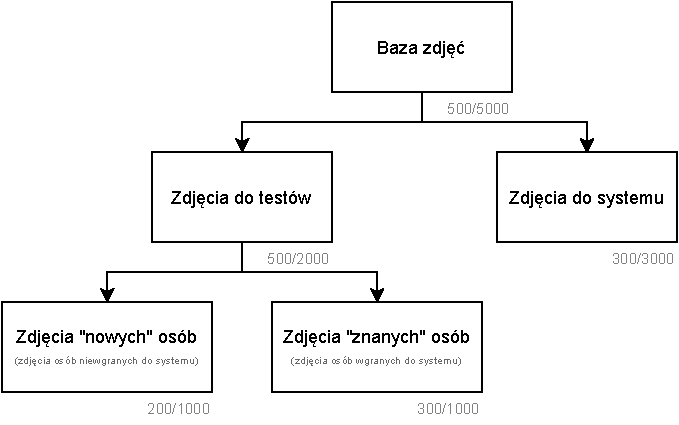
\includegraphics[width=1\textwidth]{images/podzial_zdjec}
    \caption{
        Podział zdjęć na grupy. Obok każdej z grupy widnieje liczba osób oraz suma
        wszystkich zdjęć należąca do owej grupy.
    }
    \customsource
    \label{fig:podzial_zdjec}
\end{figure}

Po podzieleniu zdjęć na grupy kolejnym krokiem jest zbadanie trafności oceny podobieństwa dla poszczególnych
progów z zakresu od \num{8} do \num{12}.
Zakres ten będzie badany z dokładnością do \num{0.1}.
Kroki, jakie zostały wykonane w badaniu, są następujące:

\begin{enumerate}
    \item wygenerowanie wektora cech dla wszystkich zdjęć z każdej grupy,
    \item wgranie wygenerowanych wektorów z grupy ``Zdjęcia do systemu'' do systemu,
    \item pobranie zdjęć z grupy ``Zdjęcia nowych osób'' i przepuszczenie ich przez
    funkcję oceniająca podobieństwo na podstawie wgranych zdjęć do systemu dla danego ``x'',
    \item powtórzenie kroku trzeciego dla zdjęć z grupy ``Zdjęcia znanych osób'',
    \item potwórzenie kroku trzeciego oraz czwartek dla nowego parametru ``x''.
\end{enumerate}

Dla kroku trzeciego, przy założeniu, że skuteczność oceny podobieństwa była by stuprocentowa, funkcja
powinna zwrócić zawsze wartość \textit{False}, ponieważ \textbf{żadna} z osób przedstawiona
na zdjęciach z grupy ``Zdjęcia nowych osób'' nie znajduje się w systemie.
Dla kroku czwartego, w przeciwieństwie do kroku trzeciego, funkcja ta powinna
zawsze zwrócić \textit{True}, ponieważ \textbf{każda}
osoba przedstawiona na zdjęciu z grupy ``Zdjęcia znanych osób'' znajduje się w systemie.
Niestety z przeprowadzonych wcześniej badań (rysunek~\ref{fig:wykres_najmniejszych_odleglosc_wspolny}) wynika,
że taki scenariusz nie jest możliwy i z tego powodu należy znaleźć taką wartość parametru ``x'',
dla którego trafność walidatora oceniającego podobieństwo będzie maksymalne.

Wyniki opisanego wcześniej badania zostały przedstawione na rysunku~\ref{fig:tranosc_walidatora_per_prog}.
Na jego podstawie można zauważyć, że trafność walidatora
rośnie wraz ze wzrostem wartości progu aż do momentu osiągnięcia
przez ``x'' wartości \num{10.2} po czym nastepuje spadek.
Dla wartości \textbf{10.2} trafność funkcji została oceniona na poziomie \textbf{92.3\%}.
Obliczony wartość oznacza, że jeżeli odległość pomiędzy dwoma wektorami, które leżą najbliżej siebie,
jest mniejsza niż \num{10.2} to system uzna, że owe wektory dotyczą tej samej osoby,
przez co proces będzie kontynuowany.
W przeciwnym wypadku zostanie rzucony błąd z informacją, że osoba przedstawiona na zdjęciu,
która podlega weryfikacji, nie jest znana systemowi.

\begin{figure}[]
    \centering
    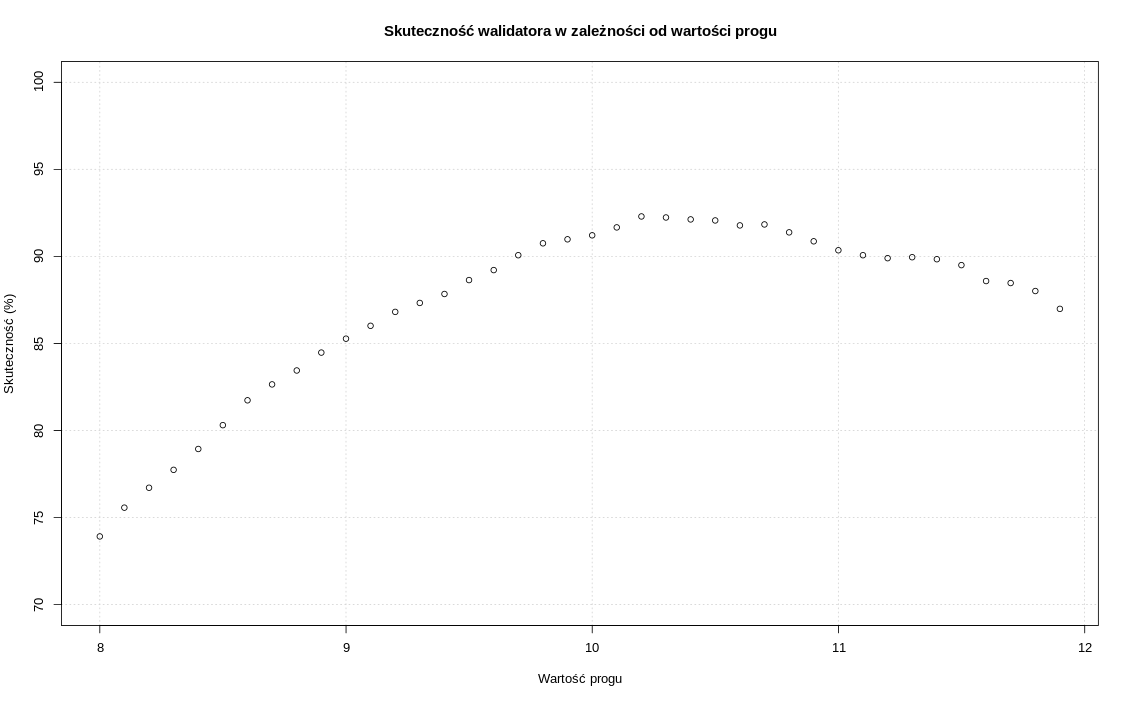
\includegraphics[width=1\textwidth]{images/trafnosc_walidator_a_prog}
    \caption{ Trafność walidatora w zależności od wartości progu (parametru ``x'') }
    \customsource
    \label{fig:tranosc_walidatora_per_prog}
\end{figure}

\pagebreak


\section{Klasyfikator}

Ostatnim krokiem w procesie działającym po stronie serwera (rysunek~\ref{fig:schemat_blokowy_systemu})
jest wykonanie klasyfikacji.
Na tym etapie wiadome już jest, że wektor cech, który trafił do klasyfikatora, reprezentuje osobę,
która jest znana systemowi.
Jest to bardzo istotna informacja, ponieważ w przeciwnym wypadku klasyfikator
mógłby dokonać klasyfikacji pomimo tego, że dana klasa (w tym wypadku osoba) nie istnieje w systemie,
co oznaczałoby zawsze błędną klasyfikację.

Do wykonywania klasyfikacji został wykorzystany klasyfikator SVM z liniowym jądrem z parametrem $C$ równym $1.0$.
Jego trafność na opisanym wcześniej zbiorze (rysunek~\ref{fig:podzial_zdjec}) wyniosła \textbf{96.1\%}.
Z powodu tak wysokiej trafności nie były testowane inne klasyfikatory.
Implementacja klasyfikatora SVM została zaczerpnięta z biblioteki \textit{sklearn}~\cite{sklearn_api}.


\section{Strona internetowa}

Zaprojektowana strona internetowa składa z prostego formularza.
Na stronie został umieszczony przycisk, który umożliwia wybranie zdjęć z dysku urządzenia klienta.
Po wybraniu zdjęcia pojawi się jego podgląd, po czym plik jest wysyłany na serwer.
Po uzyskaniu odpowiedzi z serwera zostanie wyświetlony otrzymany komunikat.
Wygląd strony zostaw przedstawiony na zdjęciu~\ref{fig:ja}.

\begin{figure}[H]
    \centering
    \includegraphicswithborder[width=1\textwidth]{images/wyglad_frontowa_aplikacji}
    \caption{Wygląd strony internetowej po wybraniu zdjęcia z dysku i uzyskaniu odpowiedzi z serwera}
    \customsource
    \label{fig:ja}
\end{figure}

    \chapter{Testowanie systemu}

Testowanie napisanej aplikacji będzie polegać na ręcznym wprowadzeniu wybranych zdjęć do systemu.
Wszystkie zdjęcia twarzy, użyte do testowania aplikacji, zostały pobrane ze zbioru CelebA~\cite{microsoft-2020-celeb1m}.
Wybrane zdjęcia (rysunek~\ref{fig:zdjeciadotestow}) zostały podzielone na dwie kategorie:

\begin{itemize}
    \item zdjęcia, które trafią do systemu jako wzorzec,
    \item zdjęcia, które zostaną wykorzystane w celu zbadania zachowania oraz trafności
    komunikatów zwracanych przez system.
\end{itemize}

\begin{figure}[H]
    \centering
    \includegraphicswithborder{images/zdjeciadotestow}
    \caption{Użyte zdjęcia do przetestowania systemu. Obok każdej grupy przedstawiona jest etykieta zdjęć.}
    \customsource
    \label{fig:zdjeciadotestow}
\end{figure}

\pagebreak


\section{Wgranie zdjęć do systemu}

Aplikacja udostępnia dla administratorów panel, za pomocą którego jest możliwe wprowadzenie
zdjęć do systemu z poziomu przeglądarki.
Po zalogowaniu się zostały wprowadzone wyżej przedstawione zdjęcia (rysunek~\ref{fig:zdjeciadotestow}).
Dla etykiety oznaczonej numerem jeden zostało wprowadzone jedno zdjęcie,
oznaczonej numerem dwa - dwa zdjęcia przedstawiające tę samą osobę, dla kolejnej trzy.
Podgląd wprowadzonych zdjęć oraz wykadrowanych twarzy został przedstawiony na rysunku~\ref{fig:po_wprowadzeniu}.

\begin{figure}[H]
    \centering
    \includegraphicswithborder{images/po_wprowadzeniu}
    \caption{ Podgląd wprowadzonych zdjęć do systemu. }
    \customsource
    \label{fig:po_wprowadzeniu}
\end{figure}

\pagebreak


\section{Zdjęcie niezawierające twarzy}

Po wysłaniu zdjęcia na serwer, zgodnie ze schematem przedstawionym na rysunku~\ref{fig:schemat_blokowy_systemu},
pierwszym krokiem jest kadrowanie twarzy.
Informacja na temat samego kadrowania nie jest znana użytkownikowi końcowemu, natomiast w przypadku,
gdy zostanie wysłane zdjęcie niezawierające twarzy, to użytkownik powinien dostać informację zwrotną.
W celu sprawdzenia, czy funkcjonalność zadziała prawidłowo, zostało wysłane na serwer zdjęcie, które zawiera krajobraz.
Z powodu, że na zdjęciu nie ma przedstawionych żadnych osób, system powinien zwrócić informację o błędzie.
Wynik testu został pokazany na rysunku~\ref{fig:wprowadzona_natura}.
Komunikat o braku twarzy został zwrócony, co oznacza, że system zachował się poprawnie.

\begin{figure}[H]
    \centering
    \includegraphicswithborder{images/wprowadzona_natura}
    \caption{ Zachowanie systemu po wprowadzeniu zdjęcia niezawierającego twarzy. }
    \customsource
    \label{fig:wprowadzona_natura}
\end{figure}


\section{Zdjęcie osoby nieznanej systemowi}

Kolejnym krokiem do przetestowania jest sprawdzenie czy system zwróci informację,
gdy zostanie wysłane zdjęcie osoby, która nie została wcześniej zaimportowana.
Z tego powodu system powinien zwrócić informację, że nie rozpoznano osoby na zdjęciu.
W tym celu zostały przygotowane zdjęcia mężczyzn oznaczone etykietą ``4'' oraz ``5'' (rysunek~\ref{fig:zdjeciadotestow}).
Wyniki testu zostały przedstawione na rysunku~\ref{fig:rezultat_nieznane}.
Dla każdego ze zdjęć został zwrócony komunikat z informacją, że nie rozpoznano osoby na zdjęciu.
Oznacza to, że system zachował się poprawnie i test można uznać za zaliczony.

\begin{figure}[]
    \centering
    \includegraphicswithborder{images/rezultat_nieznane}
    \caption{ Zachowanie systemu po wybraniu zdjęć nieznanych systemowi }
    \customsource
    \label{fig:rezultat_nieznane}
\end{figure}


\section{Zdjęcie osoby znanej systemowi}

Ostatnim krokiem w procesie jest klasyfikacja,
czyli zwrócenie informacji kto został przedstawiony na przesłanym zdjęciu.
W celu dokładniejszego przetestowania napisanej funkcjonalności specjalnie
w tym celu zostały wgrane do systemu zdjęcia osób
o różnej liczbie (rysunek~\ref{fig:po_wprowadzeniu}),
aby sprawdzić, czy wpłynie to na otrzymane wyniki.
Wyniki testu zostały przedstawione na rysunku~\ref{fig:rezultat_znane}.
Komunikaty zwrócone przez system dla zdjęć reprezentujących etykiety ``2'' oraz ``3'' są poprawne.
Dla jednego ze zdjęć przedstawiających osobę o etykiecie ``1'' system zwrócił informacje,
że nie rozpoznano osoby na zdjęciu.
\textbf{Najprawdopodobniej} spowodowane jest to tym, że w systemie znajduje się
tylko \textbf{jedno} zdjęcie reprezentujące etykietę ``1'' przedstawiające kobietę o ciemnym kolorze włosów,
a zdjęcie, dla którego system zwrócił błędny komunikat, przedstawia tę samą kobietę, tylko że w innym kolorze włosów.
Dodatkowo zdjęcie twarzy zrobione jest z inne profilu,
częściowo zasłoniętego przez włosy (rysunek~\ref{fig:porownanie_etykiety_1}).

\pagebreak

\begin{figure}[H]
    \centering
    \includegraphicswithborder{images/rezulat_znane}
    \caption{
        Zwrócone komunikaty dla wybranych zdjęć.
        Obok komunikatu została przedstawiona etykieta, którą powinien zwrócić system.
    }
    \customsource
    \label{fig:rezultat_znane}
\end{figure}


\begin{figure}[H]
    \centering
    
\includegraphics[width=0.6\textwidth]{images/porownanie_etykiety_1}
    \caption{ Porównanie zdjęcia wgranego do systemu ze zdjęciem źle zakwalifikowanym przez system. }
    \customsource
    \label{fig:porownanie_etykiety_1}
\end{figure}


    \chapter*{Podsumowanie}
\addcontentsline{toc}{chapter}{Podsumowanie}

Architektura FaceNet znakomicie sprawdza się do zadań związanych z rozpoznawaniem twarzy.

Wektor cech, które jest generowane przez sieć FaceNet

Policzona maksymalna odległość pomiędzy zdjęciami, która może wystąpić,
aby porównywane zdjęcia twarzy były uznane za podobne to \num{10.2}.
Przy takiej długości została osiągnięta maksymalna trafność samego walidatora.
Pomyłka walidatora będzie oznaczać, że osoba, która w rzeczywistości nie znajduje się w obecnej bazie zdjęć,
zostanie zakwalifikowana do następnego etapu i zostanie dokonana kwalifikacja (wynik fałszywie pozytywny).
W przypadku, gdy system zostałby użyty w miejscu, gdzie taki błąd jest niedopuszczalny, należy zmniejszyć tę odległość.
Spowoduje to, że ogólna trafność walidatora spadnie, natomiast częstotliwość występowania wyników fałszywie
pozytywnych zostanie \textbf{najprawdopodobniej} ograniczona.

Przygotowany panel administratora jest bardzo dużym ułatwieniem,
które pozwala na łatwe zarządzanie zdjęciami, które znajdują się w systemie.
Podgląd aktualnych lub dodawania kolejnych zdjęć ogranicza się tylko do paru kliknięć.
Niestety manualne wysyłanie bardzo dużej liczby zdjęć za pomocą panelu będzie wymagać dużo czasu,
dlatego w takim przypadku lepiej jest przygotować skrypt, który zaimportuje bezpośrednio zdjęcia z dysku do systemu.

Udostępniona strona internetowa pozwala na komunikowanie się z serwerem
z każdego urządzenia z internetem z zainstalowaną przeglądarką internetową.
Jeżeli urządzenia posiada aparat to jest nawet możliwość bezpośredniego wysłania zdjęcia zaraz po jego wykonaniu.
Takie rozwiązanie daje dużą swobodę w korzystaniu.


Kolejnym tematem, który nie został poruszony, jest wydajność systemu przy bardzo dużej liczbie zdjęć.
Podczas testów w systemie wgranych było 5000 zdjęć i przy takiej liczbie system odpowiadał szybko (poniżej 1 sekundy),
natomiast nie zostało sprawdzone, co się stanie, gdy liczba ta wzrośnie 10 lub 100-krotnie.



    \printbibliography[
        heading=bibintoc,
        title={Literatura}
    ]
    \listoffigures

    \newpage\thispagestyle{empty}
Imię i Nazwisko \hfill Kraków, dnia ....................\par\vspace{1cm}\par
\centerline{{\Large \bf O Ś W I A D C Z E N I E}}
\par\vspace{1.4cm}\par
Świadomy(a) odpowiedzialności oświadczam, że przedłożona praca pt.:
\begin{center}
{\sc Zastosowanie głębokiej sieci neuronowej o architekturze FaceNet
do rozpoznawania twarzy}
\end{center}
została napisana przeze mnie samodzielnie.
\par
Jednocześnie oświadczam że w/w praca nie narusza praw autorskich w rozumieniu Ustawy z dnia 4 lutego 1994 r. o prawie autorskim i prawach pokrewnych (Dz.U. z 2006 nr 90, poz.
631 z późn. zmianami) oraz dóbr osobistych chronionych prawem cywilnym.
\par
Przedłożona praca nie zawiera danych empirycznych ani też informacji, które uzyskałem(am) w sposób niedozwolony. Stwierdzam, iż przedstawiona praca w całości ani też w części nie była wcześniej podstawą żadnej innej urzędowej procedury związanej z~uzyskaniem dyplomu ani też nadania tytułów zawodowych.
\par\vspace{1cm}\par
\begin{flushright}
    ....................................... \ \ \ \ \ \ \\
    {\scriptsize (podpis)\hspace{2.3cm}\ }
\end{flushright}

\end{document}

